\documentclass[Main.tex]{subfiles} 
\begin{document}

\subsubsection{Use Case 1: Sorter klods realisering}
Sorter klods Use Casen er realiseret ved at systemet starter med at kalde ned i Data Access Layer, som muligg�r kommunikation med Robot Dll'en. Her benyttes funktionen EnterManual(), hvor der indikeres at robotten skal styres via. akser og ikke koordinater. Herefter bliver der startet en while-l�kke, som benytter funktionen MoveManual som har to parametre. Den ene s�ttes til at styre aksen, hvori transportb�ndet er og den anden angiver hastigheden p� transportb�ndet. While-l�kken er aktiv, indtil der er en klods der afbryder sensoren p� transportb�ndet. N�r dette indtr�ffer vil en variabel blive �ndret og programmet vil afbryde while-l�kken. \\
Use Casen g�r herefter brug af Use Case 1.1 og Use Case 1.2 som er beskrevet i afsnit 5.3.2 og 5.3.3. I disse include Use Cases bliver den givne klods m�lt og vejet, samt dens materialetype bestemmes.\\ 
Inden det givne materiale flyttes over til kassen, bliver der f�rst valideret om der er plads til klodsen. Hvis dette ikke er tilf�ldet bliver klodsen afleveret p� enden af transportb�ndet og k�rt ud over kanten. I tilf�ldet af der er plads til klodsen flyttes det givne materiale over til kassen, ved hj�lp af funktionerne DefineVectorCoordinates, NameAndTeachVector samt MoveLinear, som findes i Robot Dll'en. DefineVector definere den givne vektor med koordinater og NameAndTeach navngiver den og inds�tter vektoren i hukommelsen. MoveLinear bliver herefter brugt og den flytter robotarmen hen til den givne vektors koordinat. I implementeringen er disse 3 funktioner sat ind i en hj�lpe funktion(MoveRobot()), som bliver kaldt flere gange i en sekvens for at f� robotarmen til at l�gge den givne klods det rigtige sted. N�r klodsen er lagt p� plads flyttes robotarmen hen til et absolut punkt som angiver startpositionen for robotarmen - Use casen er derefter udf�rt og opfyldt. \\\\
\begin{figure}[H]
\centering
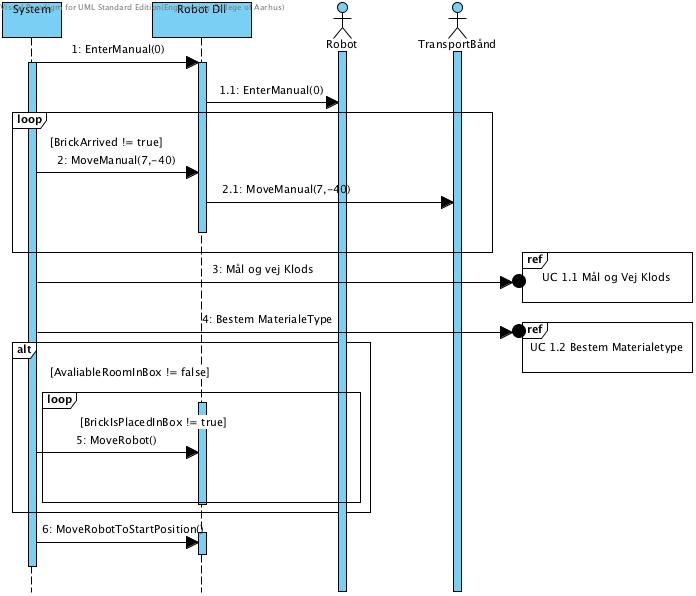
\includegraphics[scale=0.5]{Billeder/UseCaseRealiseringer/UC1.jpg}
\caption{Simpelt sekvensdiagram over Sorter Klods}
\end{figure}

\end{document}